%%%%%%%%%%%%%%%%%%%%%%%%%%%%%%%%%%%%%%%%%
% See LICENSE for licensing details
%%%%%%%%%%%%%%%%%%%%%%%%%%%%%%%%%%%%%%%%%

%----------------------------------------------------------------------------------------
%	PACKAGES AND DOCUMENT CONFIGURATIONS
%----------------------------------------------------------------------------------------

\documentclass{article}

% Package includes

\usepackage{graphicx}
\usepackage{geometry}
\usepackage{array}
\usepackage{colortbl}
\usepackage{hyperref}
\usepackage{placeins}
\usepackage{longtable}
\usepackage{multirow}
\usepackage{float}
\usepackage{caption}

\usepackage{natbib} % Required to change bibliography style to APA
\usepackage{amsmath} % Required for some math elements 
\usepackage[boxed]{algorithm2e} % required for algorithms
\usepackage{fancyhdr}
\RequirePackage{epstopdf}
\RequirePackage{tabularx}
\RequirePackage{xstring}
\RequirePackage{hyperref}
\RequirePackage{fancyhdr}

\usepackage[olditem,oldenum]{paralist}

\usepackage[xindy,toc]{glossaries}
\usepackage[xindy]{imakeidx}
% Setup margins

\setlength{\topmargin}{-0.5in}
\setlength{\textheight}{9in}
\setlength{\oddsidemargin}{0in}
\setlength{\evensidemargin}{0in}
\setlength{\textwidth}{6.5in}

% Useful macros

\newcommand{\note}[1]{{\bf [ NOTE: #1 ]}}
\newcommand{\fixme}[1]{{\bf [ FIXME: #1 ]}}
\newcommand{\todo}[1]{\marginpar{\footnotesize #1}}

\newcommand{\wunits}[2]{\mbox{#1\,#2}}
\newcommand{\um}{\mbox{$\mu$m}}
\newcommand{\xum}[1]{\wunits{#1}{\um}}
\newcommand{\by}[2]{\mbox{#1$\times$#2}}
\newcommand{\byby}[3]{\mbox{#1$\times$#2$\times$#3}}

\newlength\savedwidth
\newcommand\whline[1]{%
  \noalign{%
    \global\savedwidth\arrayrulewidth\global\arrayrulewidth 1.5pt%
  }%
  \cline{#1}%
  \noalign{\vskip\arrayrulewidth}%
  \noalign{\global\arrayrulewidth\savedwidth}%
}

% Custom list environments

\newenvironment{tightlist}
{\begin{itemize}
 \setlength{\parsep}{0pt}
 \setlength{\itemsep}{-2pt}}
{\end{itemize}}

\newenvironment{titledtightlist}[1]
{\noindent
 ~~\textbf{#1}
 \begin{itemize}
 \setlength{\parsep}{0pt}
 \setlength{\itemsep}{-2pt}}
{\end{itemize}}

\newenvironment{commentary}
{ \vspace{-0.2in}
  \begin{quotation}
  \noindent
  \small \em
  \rule{\linewidth}{1pt}\\
}
{ 
  \end{quotation}
  \vspace{-0.2in}
}

\newenvironment{samepage-commentary}
{\begin{samepage} \begin{commentary}}
{\end{commentary} \end{samepage}}

% Other commands and parameters

\pagestyle{myheadings}
\setlength{\parindent}{0in}
\setlength{\parskip}{10pt}
\sloppy

% Commands for register format figures.

% New column types to use in tabular environment for instruction formats.
% Allocate 0.18in per bit.
\newcolumntype{I}{>{\centering\arraybackslash}p{0.18in}}
% Two-bit centered column.
\newcolumntype{W}{>{\centering\arraybackslash}p{0.36in}}
% Three-bit centered column.
\newcolumntype{F}{>{\centering\arraybackslash}p{0.54in}}
% Four-bit centered column.
\newcolumntype{Y}{>{\centering\arraybackslash}p{0.72in}}
% Five-bit centered column.
\newcolumntype{R}{>{\centering\arraybackslash}p{0.9in}}
% Six-bit centered column.
\newcolumntype{S}{>{\centering\arraybackslash}p{1.08in}}
% Seven-bit centered column.
\newcolumntype{O}{>{\centering\arraybackslash}p{1.26in}}
% Eight-bit centered column.
\newcolumntype{E}{>{\centering\arraybackslash}p{1.44in}}
% Ten-bit centered column.
\newcolumntype{T}{>{\centering\arraybackslash}p{1.8in}}
% Twelve-bit centered column.
\newcolumntype{M}{>{\centering\arraybackslash}p{2.2in}}
% Sixteen-bit centered column.
\newcolumntype{K}{>{\centering\arraybackslash}p{2.88in}}
% Twenty-bit centered column.
\newcolumntype{U}{>{\centering\arraybackslash}p{3.6in}}
% Twenty-bit centered column.
\newcolumntype{L}{>{\centering\arraybackslash}p{3.6in}}
% Twenty-five-bit centered column.
\newcolumntype{J}{>{\centering\arraybackslash}p{4.5in}}

\newcommand{\instbit}[1]{\mbox{\scriptsize #1}}
\newcommand{\instbitrange}[2]{~\instbit{#1} \hfill \instbit{#2}~}
\newcommand{\reglabel}[1]{\hfill {\tt #1}\hfill\ }

\newcommand{\wiri}{\textbf{WIRI}}
\newcommand{\wpri}{\textbf{WPRI}}
\newcommand{\wlrl}{\textbf{WLRL}}
\newcommand{\warl}{\textbf{WARL}}


\makeglossaries


%\usepackage[margin=1.0in]{geometry}
%\usepackage[version=3]{mhchem} % Package for chemical equation typesetting
%\usepackage{siunitx} % Provides the \SI{}{} and \si{} command for typesetting SI units
%\usepackage{graphicx} % Required for the inclusion of images
%\usepackage{natbib} % Required to change bibliography style to APA
%\usepackage{amsmath} % Required for some math elements 
%\usepackage[boxed]{algorithm2e} % required for algorithms
%\usepackage{fancyhdr}
%\RequirePackage{epstopdf}
%\RequirePackage{tabularx}
%\RequirePackage{xstring}
%\RequirePackage{hyperref}
%\RequirePackage{fancyhdr}

%-- setup paragraphs and margins
\setlength{\parindent}{1em}
\setlength{\parskip}{1em}


%-- setup hyperlinks
\hypersetup{
  colorlinks=true,
  linktoc=all,
  linkcolor=black,
  citecolor=black,
  urlcolor=black
}
%--

\setlength\parindent{0pt} % Removes all indentation from paragraphs


\renewcommand{\labelenumi}{\alph{enumi}.} % Make numbering in the enumerate environment by letter rather than number (e.g. section 6)

\pagestyle{fancy}
\lhead{}
\chead{\textbf{SV128 Architecture Extension Specification}}  % -- classification
\rhead{}
\cfoot{} %-- format: TR YYYY-RRR-V.V; y = year; r = report; v = version
\lfoot{\textbf{SV128 0.0.1}}  % -- classification
\rfoot{\thepage}      % -- page number

%\usepackage{times} % Uncomment to use the Times New Roman font

%----------------------------------------------------------------------------------------
%	DOCUMENT INFORMATION
%----------------------------------------------------------------------------------------

\title{\textbf{RISC-V SV128 Addressing and\\Architecture Extension Specification}} % Title

%\author{John \textsc{Leidel}, David \textsc{Donofrio}, Farzad \textsc{Fatollahi-Fard}}
\date{} % Date for the report

\begin{document}

\begin{figure}
\vspace{2in}
\begin{center}

\includegraphics[width=3in]{figures/sv128.pdf} % Include the logo
\end{center}
\end{figure}

\maketitle % Insert the title, author and date

\thispagestyle{fancy}

\begin{center}
\begin{tabular}{l r}
Date: & \today \\
Version: & 0.0.1 \\ % Date the experiment was performed
Authors: & Steven Wallach\\
& John Leidel
\end{tabular}
\end{center}

\clearpage

\tableofcontents

\clearpage

%----------------------------------------------------------------------------------------
%	DEFINITIONS
%----------------------------------------------------------------------------------------
%\section*{Terms}
%\label{sec:terms}


%----------------------------------------------------------------------------------------
%       List of Figures
%----------------------------------------------------------------------------------------

\clearpage
\listoffigures
%\lstlistoflistings
\listoftables
%\listofalgorithms
\clearpage

%----------------------------------------------------------------------------------------
%	SECTION 1
%----------------------------------------------------------------------------------------
\clearpage
\section{Introduction}
\label{sec:Introduction}

\subsection{SV128 Overview}
\label{sec:SV128Overview}

This is a citation~\cite{RVSuperSPec}.

%----------------------------------------------------------------------------------------
%	SECTION 2
%----------------------------------------------------------------------------------------
\clearpage
\section{SV128 Memory Model}
\label{sec:SV128MemoryModel}


\subsection{Introduction and Philosophy}

The following is the proposal for the Operand Reference Protection System and Logical to Physical Address Mechanism for SV128.  Some of the primary motivations and underlying reasons for the structures proposed are:


\begin{itemize}
\item A logical address space greater than 64. 
\item A logical address space that is scalable to 128,  but first implementation limited to 96
\item  Whenever and where ever possible use software mechanisms used by Linux and appropriately reflected into hardware and architecture.
\item  Provide a protection mechanism based on a limited number of Domains.  Domains provide a non-hierarchical protection structure. Thus, different than Rings
\item  Provide architectural support for Virtual Machine Monitor (VMM).  VMM is part of the protection and address space translation mechanism
\item  Much of what is described is a diminutive form of the proposal for a FULL 128 bit object address space and protection mechanism.  Hopefully this will happen at one time.   The following, Figure 1A, is a  simplistic diagram of the FULL APPROACH. (Only for reference purposes).
\item  Independent of the user level ISA.  This means, if one wanted,  SV128 could be supported on, for example, INTEL and ARM processors
\end{itemize}

The format of a SV128 address space is:

\begin{figure}[h]
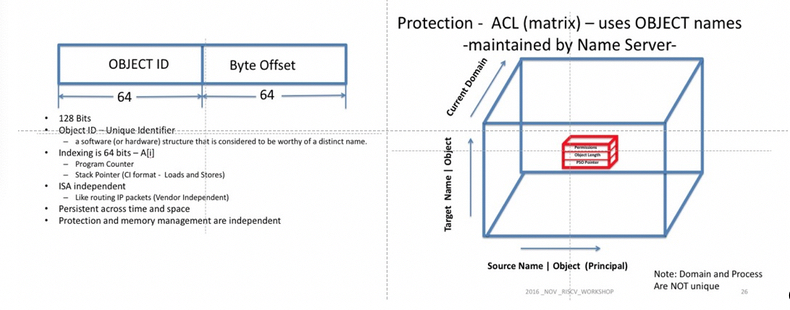
\includegraphics[scale = .4] 
{figures/figure1a.jpg}
\caption{Caption goes here for Fig1a}
\end{figure}

\subsection{SV128 Memory Protection}
\label{sec:SV128MemoryProtection}

%----------------------------------------------------------------------------------------
%	SECTION 3
%----------------------------------------------------------------------------------------
\section{SV128 Protection and Address Translation} 

This chapter specifies  the Protection and Address Translations mechanisms. When and where appropriate,  registers will be named.  At this time,  these registers are place holders. The objective of the described mechanisms is to support a hardware supported hypervisor implementation, and a limited domain based protection structure.  Additionally, a shadow stack mechanism is defined.  This permits the user to call an external library and constrain that library to  a well-defined data set as well as stack isolation.  

Additionally, in many cases,  definitions and tradeoffs follow or are heavily influenced by current Linux internal designs.   Linux running on SV128 is the target implementation. The purpose of this description is to establish the higher order mechanisms.  The actual registers and instructions follow. 

\subsection {Address Translation Overview}

Eventually more tables than currently show logical to physical translation (two sets) for an SV/128 bit virtual address, are provided.    For now, assume that this translation follows the RV64 RISC-V definitions for the 64 Object  (Byte) Offset.  Each Object Id,  indexes into a table   with the contents of this table entry denotes, among other things,  which RV64 address translation to be used.   In doing this,   it is much easier to support executable images for RV64 and RV32 binaries.  Also, Linux code will have been written that does all this for RV64.  Thus, only one more level of level of indirection is needed. It should be noted that the initial  indexing will more than likely be hashed.  This depends on how many Object Ids  are defined.

Since there are two sets of tables:  Hypervisor and No  Hypervisor.   There are two sections for logical to physical translation,  that deal with the presence or absence of a Hypervisor.

FORMAT OF LOGICAL ADDRESS SPACE

There are 2   logical address spaces that are supported on SV128 implementations.  The two are: RV64 (and RV32) for 64 bit RISC-V executable images. If these execute on a Hypervisor based system,  the page tables and protection structures need to adhere to the  structures defined for a 64 virtual address. The reason being that the kernel that is active is a 64 bit kernel and consequently creates 64  bit page tables. For native 64 bit address space applications,  the page tables and protection structures adhere to the structures defined by the SV128 architecture.



The format of a SV128 address space is:



\begin{figure}[h]
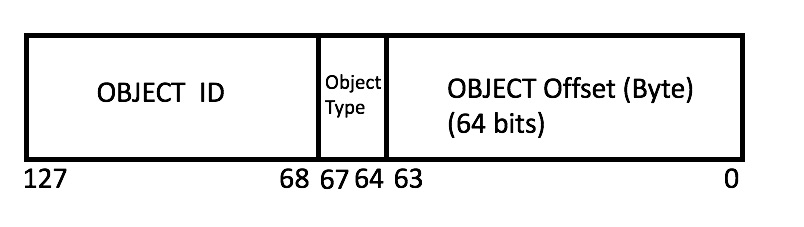
\includegraphics[scale = .4]
{figures/figure1b_objectid_image.jpg}
\caption{Caption goes here for Fig1b}
\end{figure}


Even though 64 bits are allocated for the Object ID,  the first implementation will be restricted to 32 bits.  That  means that the logical address space of SV128 is 296  bytes.  This is  very similar to current Implementations of a 64 bit logical address space.  Most, if not, all current processor designs  only support 48 to 52 bits of the logical address space.

Indexing a SV128 logical address is mod 64.  This means ONLY the Object Offset takes part in the arithmetic indexing operation.  The OBJECT ID is NOT modified in any manner during indexing.

There are several values of the OBJECT ID that have predefined meanings.  As currently defined,  the Object Types defined are: 


\begin{itemize}
\item Object  Type= 0,1,2,3 -  Kernel Object.
\item   Object  Type = 4 – Byte offset is RV64
\item   Object  Type=  5 -  Byte offset is RV32
\item   Object   Type= 6 -   Interpret Object Bits 68 thru 95 (28 bits) as a PGAS Object
\item   Object Type = 7 -    Interpret Object Bits 68 thru 95 (28 bits) as a local OBJECT ID
\item   Object  Type = 8 thru 14 reserved
\item  Object  Type- 15 – Interpret Bits 68 thru 127 (60 bits) as an Object ID

\end{itemize}

The above encoding may eventually be HUFFMAN encoded.  This would eventually permit bigger OBJECT ID for certain objects.  I expect some form of IPv6 address will be defined.

Kernel Objects are statically defined to help create a hardware implementation that is secure against speculation from user space to kernel space.  An implementation may CHOOSE to disable speculation, no matter what form it takes,  when a Kernel Object is  being referenced.  When the protection system is operating  and references to  Object 0, 1, 2, or 3,  are permitted,  an implementation may choose to support hardware speculation.  An implementation may also choose to support or disable cross object speculation when In user space.

\subsection{Protection}

This chapter describes the protection structures  for SV128.  The protection structures are defined in a manner that directly supports the following RISC-V paradigm.

\begin{center}
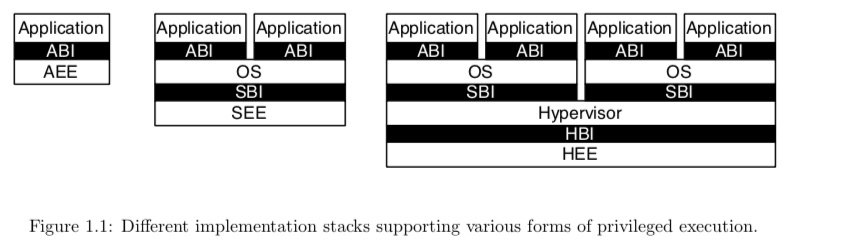
\includegraphics[scale = .4]
{figures/figure1c_riscv_stacks.jpg}
\centering
\end{center}

\begin{center}
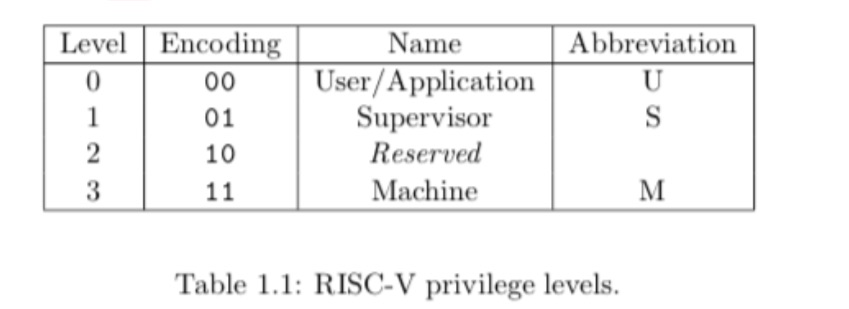
\includegraphics[scale = .4]
{figures/figure2_privleged_level_simple.jpg}   \centering
 \end{center}


Another way to depict this is  from the INTEL  VTx structures (see Figure~\ref{fig:intelvtx}).

\begin{figure}[h]
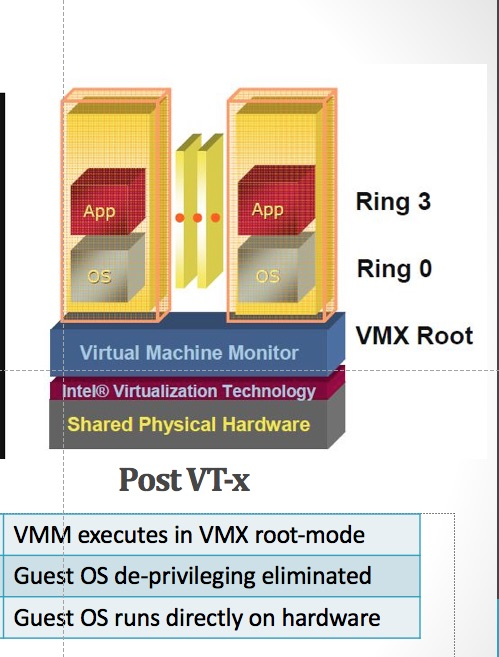
\includegraphics[scale=.4]{figures/figure2a_intelvtx.jpg}
\caption{Intel VTx structures\label{fig:intelvtx}}
\end{figure}

It should be noted,  that the static allocation of the OS to Ring 0,  by INTEL, precludes the direct incorporation of the address space and protection mechanism of Virtual Machine Monitor with the address space of the OS (noted as Rings 0 thru 3). This static allocation is appropriate for non-virtual machine monitor situations.  This is NOT the case for SV128. For SV128,  protection CONTEMPLATES a Virtual Machine Monitor.

\subsection{Domains}

The definition of SV128,  assumes from the onset,  the support of 4 non-hierarchical levels of privileged execution.  These 4 levels are:  USER/APPLICATION (Domain – 3).  SPARE,  OS (Domain -1), HYPERVISOR (Domain-0).   The definition of the protection structures is INDEPENDENT of the definition of the SV128 virtual address space.  When this virtual address space is visually examined,   as previously noted,  it is partitioned into OBJECT ID and OBJECT OFFSET. Some object enumerations may have static meanings and these meanings may have protection ramifications.  For an OBJECT ID equal all zero’s means the OS kernel object. The USER never references the Hypervisor Object. This helps  prevents various security breaches due to speculative execution. 

As will be noted the permissions of each of the 4 domains are independent of one another.  The 4 domains,  with hardware, directly supports  what is displayed in Figure 1. The objective of the creation and functioning of  these 4 domains,  is to directly support, in one homogeneous architecture, the software structures shown in Figure 1 and 2. When a memory reference is made,  access permissions as designated by the current domain are interpreted.  

While not currently implemented,  one can anticipate that over time,  the Hypervisor and OS kernel will become aware of each other.  SV128 anticipates this and consequently  defines its structures accordingly.

When the OS  or VMM is booted up,  a privileged register  (HYPER\_PRESENT) is set.  This register indicates the presence or absence of a Hypervisor.    The state of this register is used to determine logical to physical translation and other  VMM (virtual machine) operations. Various other registers are set when the VMM is booted.

Domains are defined to isolate and protect data from one part of the OS from user data.  One of the classical computer domains is RINGS.  These are hierarchical in nature.  Usually the user is in the ring that had the least privileges and the OS in the ring that had the most privileged.  Due to the hierarchical nature of rings,  various hardware implementations,  based on the definition of the logical address space exist.  Address references are mediated based on current   ring and target ring. This generally works quite will.  However, there are cases,  that the static inflexibility of this structure, leads to complex sharing structures.   Thus, for SV128 four non-hierarchical domains are defined. The OS may choose, via entries in the PTE to make data references hierarchical or not. Figure 5,  the format of a PTE shows the domain  permission fields in a PTE (4 bits).  When an address is translated from logical to physical the meaning and use of these fields will be specified.


\begin{center}
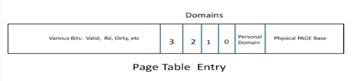
\includegraphics[scale = .9]
{figures/figure2b_pte.jpg}
\centering
\end{center}

\subsection{DOMAIN CROSSING}

Crossing a domain has to be mediated.  Arbitrary entry  points are NOT  permitted. When crossing a domain,  the domain call instruction sequence MUST access a table in the Called Domain. The base of this table is defined in a register called: DOMAIN\_ACCESS\_BASE. 

Eventually the appropriate registers and instructions will be defined, once the definition is finalized.


 Assume for description the DOMAIN call instruction has the following format:

\begin{figure}[h]
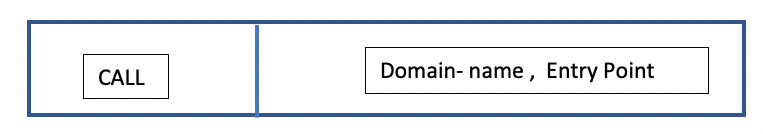
\includegraphics[scale=.4]{figures/figure3_call_instruction.jpg}
\caption{Call instruction}
\end{figure}

\subsection{Domain Access Table}

When an OS is created, either due to either a native SV128 OS or a SV128 Hypervisor,  4 registers are loaded.  These 4 registers  contain the logical address of the Domain Access Table.   These registers are called:  Domain Access Base.  (DAB). The structure of  these table is:

\begin{center}
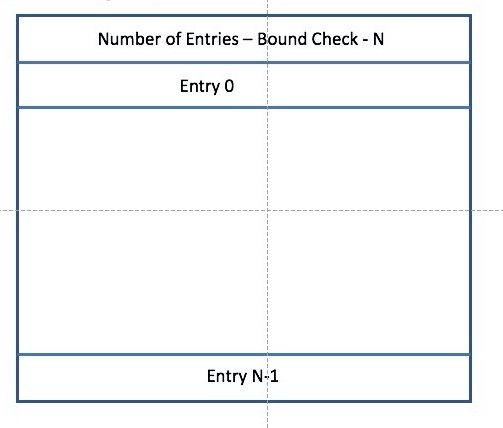
\includegraphics[scale = .4]
{figures/figure3a_table_structure_general.jpg}
\centering
\end{center}

		                 FIGURE 3A – Domain Access Table \newline
		                 
The base of this table is contained in the Domain Access Base register. \newline


		                 
		                 
		                 
		     
		                 
When domain call instruction is executed the following occurs.  The Domain Name is used to logically reference the appropriate Domain Access Register.   The first entry is used to perform a bounds check.  The entry point named  in the instruction (an integer) is compared to the Bounds Check  Value on  the Domain Access Table.  If  the specified entry point is valid,  then   the specified entry  point is used to index into the table and branch to the first location of the called routine.  There is NO OTHER WAY to transfer control from a caller to callee domain. The return domain instruction is the compliment of the CALL Domain.

In addition to these transfer of control, a new stack is created  in the called domain.  The called domain may access the caller’s domain,  but the caller’s domain cannot access the called domain’s stack.

To deal with the situation that a call, for example, from domain 3 is only permitted to domain 2, and no other domains,  the following is defined. The previously defined domain access register (DAR) besides specifying the logical address of the Domain Access Table,  also has 4 2-bit fields.  These fields are permission fields that note whether the caller can access the called  Domain Access Table.  Since Domains are NOT HIERARCHICAL in nature,  we cannot assume that, for example, domain 3 cannot call domain 1, or vice versa. 

There are 4 domain access registers (DAB).  The OS or Hypervisor is responsible for loading these registers.  The instruction used to load this register is privileged.  What a privileged instruction means is described later

CALL

When this is executed the entry, point noted in this instruction is used as an index into the table maintained in the called domain.  The index is calculated as:  index plus DOMAIN\_ENTRY\_BASE.  

The contents of this entry indicate: 
	.The index is a valid index. A bounds check is performed 
	.Can this domain be called from the caller’s domain. The CURRDOM is used for this
If the above is true,  a transfer of control, stack switching occurs.  CURRDOM is now changed to the callee’s domain. CURRDOM is a register.

RETURN

In a non-hierarchical system the return is basically the same as the call. For SV128, the supporting structures are described in Figure 1, etc.  And this is hierarchical.  Thus, the RETURN from a domain call is:  switch stacks,  change the CURRDOM to the original caller’s domain.  Since the structures are hierarchical,  it can be  assumed that the PTE’s used by an inner domain,  have access to the caller’s domain data. 

For a detailed description of domain call and return, see Appendix A.

%----------------------------------------------------------------------------------------
%	SECTION 4
%----------------------------------------------------------------------------------------
\section{Memory Translation}

\subsection{Translation of Logical to Physical Addresses}

There are two protocols for logical to  physical address translation.  One protocol is for the situation when there are only 3 domains used.  There is no Hypervisor or Virtual Machine.  The other protocol is for logical to  physical translation  when a Hypervisor or Virtual Machine is supported. The tables to translated logical to physical are straightforward in most cases.   This is especially true for the case of no Hypervisor.

When time permits,  the support for various   physical pages sizes will be specified.  Additionally, figures that show the various  page table levels will be provided.

\subsection{Translation With No Hypervisor: RV64}

The SV128 address space, though not necessarily protection, is hierarchical in nature. Figure 1.  (above) is a description of this.  Supporting this structure,  in hardware,  means that one needs to know the current address space and the  target space to be referenced. As part of the machine state (a register),  will be provided that denotes the current domain. For purposes of this description,  this 4 bit register is called: CURRDOM.   There are 4 domains.  Each domain is independent from one another.  There is NO implied hierarchical  ordering implied. (UNLIKE  RINGS).  Each domain has its own access bits (e.g., Rd, Wr, Exec, TBD). There are well defined calling and return protocols when a domain is called or returned.  Defining protection In this manner permits more extensible and opened protection mechanisms to be developed.  

The following is the  translation for RV64 of the current RISC-V ISA.  I am using this to describe what is appropriate for SV128.   The page table structure of the translation of a 48 bit virtual address for RV64 is:


\begin{figure}
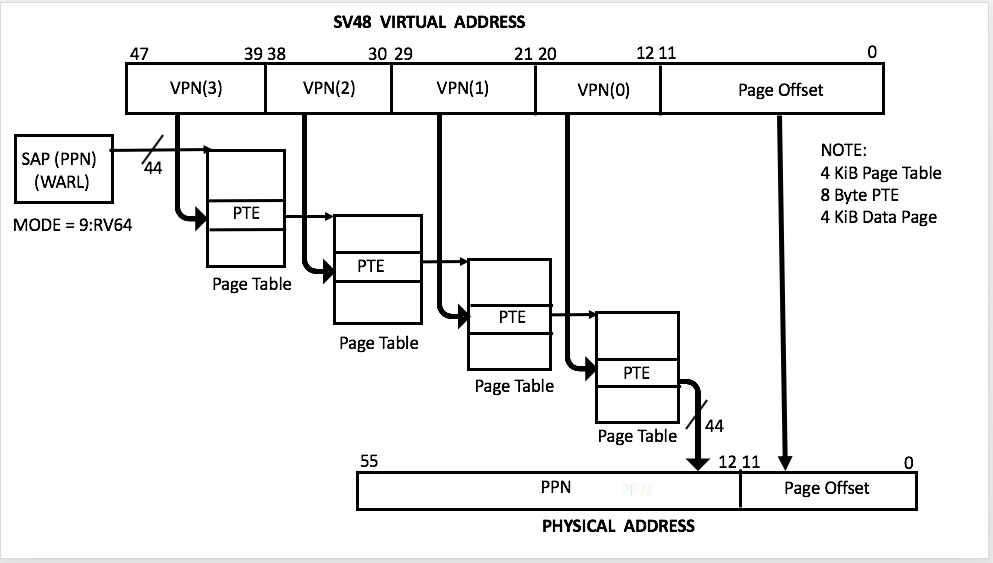
\includegraphics[scale=.4]{figures/figure4_sv48_translation.jpg}
\caption{CURRENT RISC-V TRANSLATION OF VIRTUAL TO PHYSICAL – SV48}
\end{figure}

\section{Translation With No Hypervisor: RV128}

For SV128 the address of the page table comes from an index (hash) of the Object ID of the  128 bit virtual address).  Thus, what is noted as SAP (PPN – WARL) for RV64 is replaced by this  hash. 

The hashed Object ID is used as an index into the Domain\_Address\_Translation Table (DATT).  The base of this table (on physical memory) is contained in the Domain\_Translation\_Base register  (DOMTRANBASE). There is one DOMTRANBASE register per domain.  Each domain has its own address translation base register.

%               OBJECT_ID (HASHED)
         
\begin{figure}
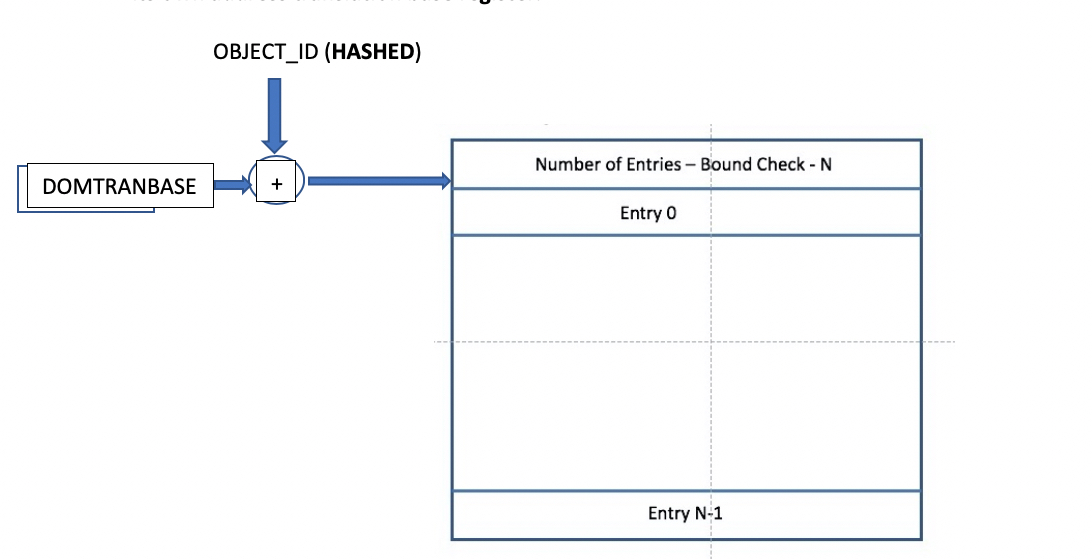
\includegraphics[scale=.4]{figures/figure4a_datt_translation_table.jpg}
\caption{Domain\_Address\_Translation\_Table (DATT)}
\end{figure}

The contents of a valid indexed entry indicate:  Valid/Not Valid, Type of Translation -  RV64 or RV32,  page table structure,  page size.  And finally, the physical address of the first page table. We should consider a DIRECT referenced to a data item without needing a page table.  In essence a valid indexed entry IS A PTE. There may be OTHER  flags and other data fields.  Among the possibilities are:  bonds check on the 64 bit virtual address,  some characteristic   the data referenced, data is encrypted, etc.


When a data or procedure call is executed,  the CURRDOM is used to determine if the reference is valid (CURRDOM selects one of the four domains in the PTE).  This is implemented by defining various fields in a Page Table Entry  (PTE) that references the desired operand.  The following discussion pertains to the interpretation of the final PTE (the one that references data or code)


The Format of a PTE (denoted as VPN (0) is the above figure) is:

\begin{figure}
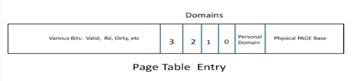
\includegraphics[scale=.8]{figures/figure2b_pte.jpg}
\caption{PAGE TABLE ENTRY}
\end{figure}

Each of the above domain fields is 4 bits wide.  These 4 bit indicate permissions (or lack thereof) for READ,  WRITE,  EXECUTE,  TBD. (perhaps reduce to 3 later on). One possibility for the unused bit to trap to a routine that mediates the access in some controlled  manner (like time of day)

\begin{center}
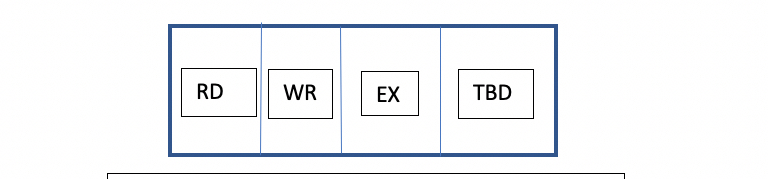
\includegraphics[scale=.4]
{figures/figure5a_domain_permissions.jpg}
\centering
\end{center}

Assume the LOAD instruction is executed.  The load instruction generates a SV128 virtual address.  This virtual address needs to be translated to a physical address.  Only for purposes of this description, assume that we have translated the virtual address and now have accessed the final PTE needed to reference the desired operand (data or procedure), as shown in Figure 5 Page table Entry.   The following now occurs.  The value in the CURRDOM register is compared to the corresponding domain field of this PTE.   If a read is requested the read permission bit is examined.  If a read is authorized,  the referenced operand is fetched.  If a write is requested,  the write permission bit is examined.  If a write is authorized the referenced operand is written.  If a transfer of control is requested,  the execute permission bit is examined.  If  a transfer is authorized,  a transfer of control happens.  The CURRDOM is not  CHANGED.

The domain access permission bits for intermediate page table entries are NOT interpreted.   Only for the final PTE permission bits that references the operand  are interpreted.

%----------------------------------------------------------------------------------------
%	SECTION 5
%----------------------------------------------------------------------------------------
\section{Shadow Stack}
SHADOW  STACK/SANDBOX (PERSONAL DOMAIN)

PARAPHASING  a phase from Greek Mythology: Beware of GEEKS Bearing Gifts

Protection comes in many forms.  The most dominant form is protection of  the OS Kernel/VMM from user access. This is generally supported via the definition of instructions that  can only be executed by the Operating System.  This assists in separating user data and control from OS  data and control.  In contemporary protection systems one would also like to provide a similar level to the USER.  this is the case, when the USER calls an externally provided software routine,  a library call. In a manner similar to the OS/USER structure, SV128 provided a level of library isolation and control via the creation of a SHADOW STACK  and with mediated operand access by the library to the caller's data (SANDBOX).

The characteristics of the shadow stack are:  A separate set of subroutine control registers (SP and FP),  and an additional domain field in the PTE.  In essence a PERSONAL DOMAIN, for the user is defined and hardware supported.  This functions is as follows.

The user executes the subroutine call instruction.  When the address of the called routine is translated (using defined entry points as in a domain call), using the Domain Translation Base register of the CURRENT DOMAIN)  the PERSONAL DOMAIN bits of the final PTE are interpreted. If the appropriate bit is set,     a shadow stack call is initiated. This results in a new set of stack management registers.  The callers stack management registers are NOT  accessible to the called routine.

This also now means,  that the  address translation of the memory references from the called routine  NOW INTERPRET  the personal domain bits of the PTE.  (The translation space is still the caller’s space).Thus, no new PTE translation tables are required.   In this manner, the USER (the caller) can indicate that its data structure is only read only or no access (SANDBOXING on a page basis).  When the called routine exits from the call (a return),  the caller stack management registers are used.  Thus, the called routine, with these hardware enforced features,   is restricted to particular caller defined data references and return control This is similar to the mechanisms provided to protect and mediate the interactions between and OS kernel/VMM.  But now extended,  in a limited manner to the USER.




For example,  assume the user has 1 GByte of data managed by a RV64 address space for one object.   The page tables indicate the physical location and permission bits for this 1 GByte of data.  The user calls a library that it wishes to be SANDBOXED and permission to only read one particular 4Kbytes of data.   Prior to the call,  the user makes a sys\_call.  The sys\_call results in an entry point for the called routine being created in the Domain Address Translation Table.  Additionally, the PTE for the referenced page is marked for the appropriate permissions in the PERSONAL DOMAIN field. All other permission bits are disabled.  Thus, the called routine can only read/write the specified 4 Kbyte page,  even though the library is in the same domain and uses the same page tables.

The Shadow Stack is depicted in Figure~\ref{fig:shadowstack}.


\begin{figure}
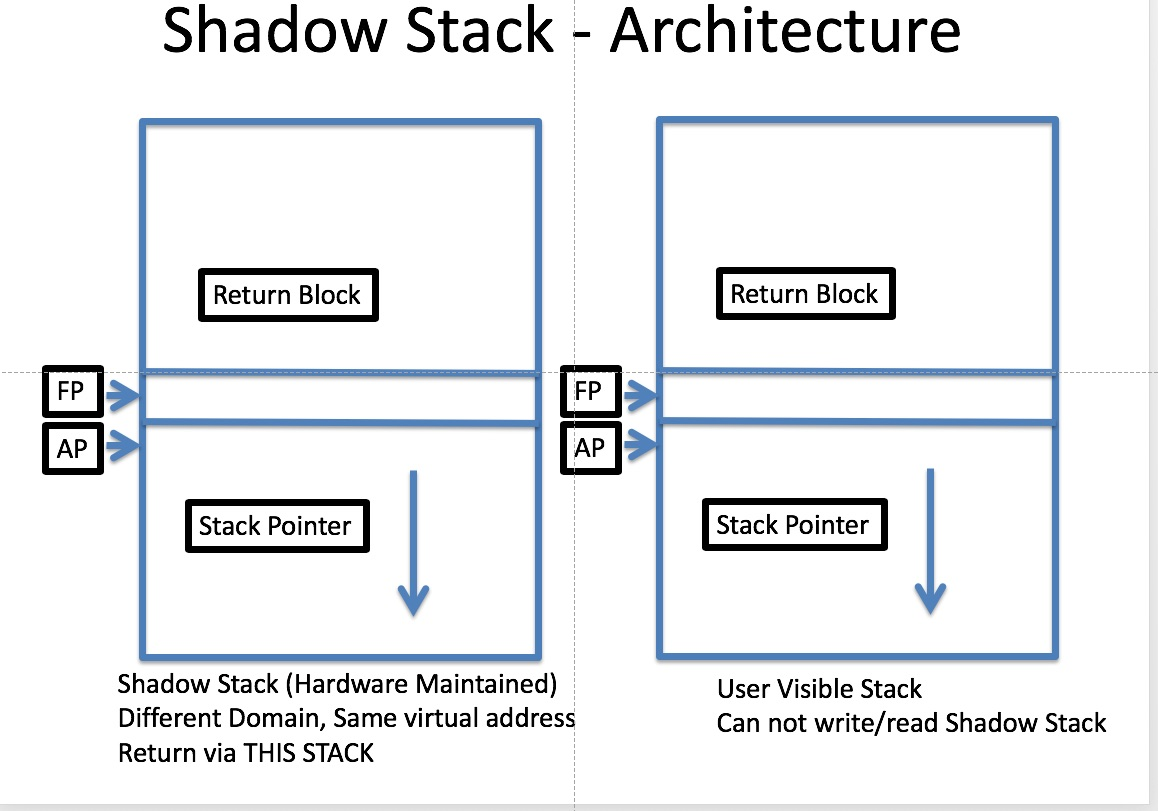
\includegraphics[scale = .4]
{figures/figure6_shadow_stack.jpg}
\caption{SHADOW STACK - ARCHITECTURE\label{fig:shadowstack}}
\end{figure}

%----------------------------------------------------------------------------------------
%	SECTION 6
%----------------------------------------------------------------------------------------
\section{Logical to Physical Address Translation with a Hypervisor}


This is, perhaps the most difficult   protocol to support in hardware.  The reason is simple,  the OS thinks it manages ALL of physical memory.  But there  are multiple OS’s.  Thus, if this was allowed in some uncontrolled manner, there would be conflicts for physical memory allocation. In many cases,  additional registers are defined.  These registers, in many cases,  directly support VMM.  The objective for SV128 is minimizing the overhead of VMM which results in minimum performance degradation relative to non-vmm systems.

\subsection{Problem Statement}

The GuestOS in Figure~\ref{fig:guest-logical-physical} creates the page tables for its users.  The GuestOS assumes it has TOTAL control of the physical memory actually implemented (as it would normally have).  Thus, is allocates physical memory and  consequently fills in PTE’s for a user process accordingly.    To make this work, with multiple OS’s,  the VMM needs to allocate subsets of physical memory to each running OS.  For example,  assume there is 32 GBytes of physical memory.  Also, there are 4 executing GuestOS’s.  The Hypervisor could allocate physical memory as follows (ignoring overheads).  16 GByte to GuestOS \#1.  8 GByte to GuestOS\#2,  and 4 GByte to GuestOS\#3 and OS\#4. Thus the 32 GBytes pf physical memory is allocated.  

There are several consequences of the above.  Each GuestOS has to know how much physical memory it is allocated.  Let’s assume this is in a register called:  OS\_PHYS\_MEMORY (OSPHYMEM).   Only the OS and VMM can modify this register.  However, when each GuestOS creates page tables for its users,  it assumes that physical memory starts form ZERO.  You cannot, in this example,  have each OS allocating pages from physical address ZERO. Thus, the physical address’s in each GuestOS page tables  somehow have to be redirected or not used. So how do we do this? One way is to always redirect physical address when a VMM is present.  That works but adds incredible about of overhead for logical to physical translation.  In essence each translation step requires 2 steps.  Another  method,   called a SHADOW or NESTING approach is what will be supported.  There are several mechanisms that need to be defined for this to work.

Using the translation of RV32 the following is defined. (for describing only)

\begin{figure}
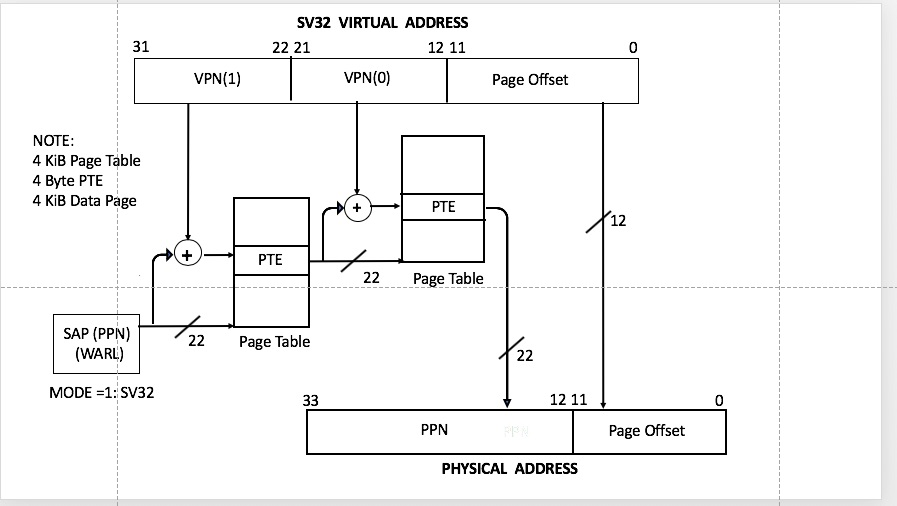
\includegraphics[scale = .4]
{figures/figure7_rv32_pte.jpg}
\caption{GuestOS created page tables for translating logical to  physical (OS Physical Address Space)\label{fig:guest-logical-physical}}
\end{figure}


The VMM creates the following


\begin{figure}
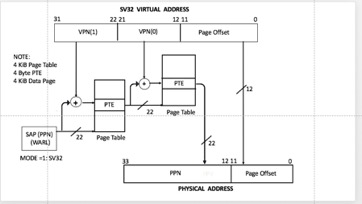
\includegraphics[scale = .9]
{figures/figure8_hypervisor_page_table.jpg}
\caption{Hypervisor  page tables for translating logical to physical (VMM Physical Address Space)}
\end{figure}

There is a VMM status  control register.  When VMM is enabled this results is the following: The base register for address translation for RV32 is changed from SAP (PPM WARL)  to the VMM\_REG. 

 In reality, as a result of a physical address base for each domain,the VMM\_REG becomes the   Domain Address Translation Table (DATT) Base   register.  This register can only be changed when the current domain is 0, when a Hypervisor is present.


 The Hypervisor created page tables, in the VMM address space are NOW used (Figure 8), in place of the GuestOS created page tables for logical to physical  translation.   In essence the overhead for a VMM logical to physical  translation is substantially reduced.   The indirection previously described is reduced to ONE indirection, once upon   initiation of lookup,  rather than for all physical memory references external to the VMM. This approach is NOT NEW and has been implemented in several systems.

In essence the GuestOS created page tables are made redundant.  When these tables are initially created by the GuestOS,   the instructions used are trapped to the VMM.  We need to define what privileged instructions are executable in domain 1 and domain 0.  (thus, one benefit of the domain protection system). In this way,  the Hypervisor knows what the GuestOS is doing, but in allocates REAL physical pages.  The GuestOS allocation of physical pages is  meaningless with respect to real physical memory addresses. Thus, the PTE’s created by the Hypervisor are IDENTICAL to the PTE’s created by the OS, OTHER than physical address’s.  

We need to consider at least one more item.  The user requests more memory from the GuestOS, during the running of the application. ( MALLOC).  For normal GuestOS running,  once memory is allocated or deallocated the appropriate PTE’s are modified (indicating valid PTE for new data, or invalid PTE for deallocated date). How do we do this, in the case of VMM and the OS page tables are meaningless?   How do we make changes in a PTE when an application is running?

The following works for this situation.  Assume we need to modify the PTE’s of VPN(1) and VPN(0) of the logical address space  to correctly execute the allocation or de-allocation of physical memory. We need to know one more item.  When the GuestOS is booted for the first time,  it establishes a correspondence  between virtual and physical memory. (Figure 9 and 10). This correspondence is as follows.  If there is 32 GBytes of physical memory,  the first 32 GBytes of Virtual Address Space of the Hypervisor is statically allocated  to this virtual to physical  mapping. Meaning when the VMM runs in virtual addressing mode,  it addresses ITS OWN memory mapping as virtual equals physical.  The same mapping is done for the GuestOS in domain 1.  But in this case, only for the physical memory allocated by the Hypervisor. (For Example, OS\#1 – 16 GBytes out of a possible 32 GBytes).

This means that a GuestOS (not VMM) physical address is actually a mapped virtual address spanning the physical memory allocated to the OS by the Hypervisor.  Thus, if we know when the GuestOS is referencing this memory,  we can redirect the translation  to the Hypervisor  to the real physical address or in this case, a PTE (Remember a PTE is always physical addressed.  Something have to be real).  

How do we do this?  We know the physical memory allocated to the GuestOS by the Hypervisor.  Let’s call this PHYSICAL MEMORY.   Under normal operation,  any user virtual address uses the Hypervisor created page tables.  So, we need to know when the GuestOS  references what it believes to be physical memory.   This is  accomplished in the following manner. 

As previously described,  the GuestOS kernel references the page table using a virtual address.  As with a user vertical address,  this GuestOS kernel virtual address is translated using the page table in the Hypervisor address space (Kernel 0).  When these page tables are created ALL the PTE’s are labeled READ ONLY.  Thus, any attempt to modify the contents of a user page table (in the VMM space),  by the GuestOS is trapped.  This trap is vectored into the Hypervisor space.

The consequence of all this results is the following.  Any and all GuestOS (Domain 1) actions that access and/or modify the PTE’s of the processes it manages are redirected to the PTE’s maintained by the Hypervisor in Domain 0.  There is no loss in performance during the normal execution of an application.

The following figures are used to explain this mapping of physical to virtual for the kernel.

\begin{figure}
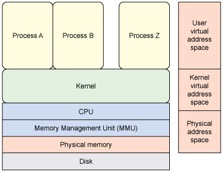
\includegraphics [scale = .4]
{figures/figure9mapping_logical_physical.jpg}
\caption{MAPPING OF PHYSICAL TO LOGICAL ADDRESS SPACE}
\end{figure}


FIGURE  9  - 
\newline
\newline

\begin{figure}
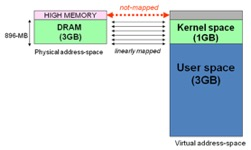
\includegraphics[scale = .4]
{figures/figure10_kernel_physical.jpg}
\caption{VIRTUAL ADDRESS SPACE AND KERNEL PHYSICAL ADDRESS SPACE}
\end{figure}


%----------------------------------------------------------------------------------------
%	SECTION 7
%----------------------------------------------------------------------------------------
\section{TLB Architecture and Discussion}

While  various approaches can be discussed and descripted,  there is one TLB characteristic that is the most important,  the working set size managed.   Thus, if there is a 32 GBytes of physical memory,  the working set of the TLB must be at least 32 GBytes.  This has to be true even for small page sizes.

The next feature always discussed is the associativity approach.  Meaning does the TLB have to be purged after each process switch or not?   If not purged how is some level of global uniqueness maintained.  For SV128,  knowing that virtual address are created from domains, provides one type of uniqueness.    For the first implementations,   the use of the Linux Unique PID (32 bits) may be a good and rational choice.  This would be true if we choose a NON purge strategy when we have process multiplexing.

Before a description of 3 possible TLB architectures,  the following is how Linux views the virtual address of current 64-bit virtual address architectures.

\begin{figure}
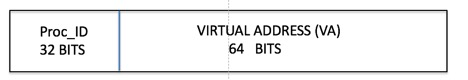
\includegraphics[scale = .7]{figures/figure11_linux_kernel_address.jpg}
\caption{VIRTUAL ADDRESS SPACE MANAGED BY THE 64 BIT LINUX KERNEL}
\end{figure}



Linux maintains up to 232  process  id encodings.  Linux attempts to assign a global unique name.  Linux manages this table for name allocation,  name  revocation, etc.  

The possible TLB architectures are:

One implementation is to associate only a 64 bit virtual address.  This means the TLB only has the working set of ONE PROCESS.  Thus, upon process multiplexing,  the TLB must be purged.  This is the simplest  implementation.

The second  implementation is to associate on the 96 bit kernel managed virtual address.  Thus, upon  process multiplexing  there is no need to purge the TLB.  The tradeoff is higher performance and lower TLB page walking when multiple processes are switching.


The third implementation is only relevant when a VMM is present.  As noted before the Linux  created and managed 96 virtual address is  unique for  the case where there is only one Linux kernel.   When there is a VMM,  this is not the case.  So how can, if we want, create a TLB that DOES NOT have to be purged when there is multiplexing among Linux kernels?  This can be done by appending the PHYSICAL address of the page tables created by the Hypervisor for each instance of a Linux kernel.  By definition the physical address of the page tables for each Linux kernel base to be unique.  Define this entity (in a register) 	PHYSICAL KERNEL BASE (assume 40 bits). This is the register noted as VMM BASE in Figures 7 and 8.    Thus if one wants to create a TLB that is unique for ALL instantiations of all Linux kernels,  the virtual address that is associated has the following structure. 

\begin{figure}
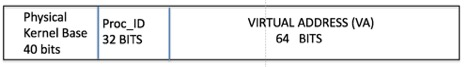
\includegraphics [scale = .7]
{figures/figure12_address_tlb_lookup.jpg}
\caption{Address used for TLB Lookup}
\end{figure}

%----------------------------------------------------------------------------------------
%	SECTION 8
%----------------------------------------------------------------------------------------
\section{ISA and Traps/Faults}

The stardard risc-v isa is supported in SV128.  The  general registers are extended to 128 bits. There will be several instructions defined that deal with domain crossing.  Instructions that load and store the various previleged resgiters will also  need to be defined.  Once there is agreement on the logical address and  protection mechanisms,  these instructions will be defined.

There are two possible approaches to the handling of traps, daults,  and interrupts.  One approach is to extended the RV64 definiton to  accomodate 128 bit pointers.  The other approach is to define a  different paradigm.











%----------------------------------------------------------------------------------------
%	SECTION 9
%----------------------------------------------------------------------------------------
\clearpage
\section{SV128 Machine Organization}
\label{sec:SV128MachineOrganization}

%----------------------------------------------------------------------------------------
%	SECTION 10
%----------------------------------------------------------------------------------------
\clearpage
\section{SV128 Instruction Set Extension}
\label{sec:SV128InstructionSetExtension}

%----------------------------------------------------------------------------------------
%	SECTION 11
%----------------------------------------------------------------------------------------
\clearpage
\section{SV128 Instruction Set Listings}
\label{sec:SV128InstructionSetListings}

%----------------------------------------------------------------------------------------
%	ACKNOWLEDGEMENTS
%----------------------------------------------------------------------------------------
\newpage
\section*{Acknowledgements}
\label{Acknowledgements}
\addcontentsline{toc}{section}{Acknowledgements}

External acknowledgements go here

%----------------------------------------------------------------------------------------
%	REFERENCES
%----------------------------------------------------------------------------------------
\newpage
\addcontentsline{toc}{section}{References}
\bibliographystyle{plain}
\bibliography{sv128-arch-spec}

%----------------------------------------------------------------------------------------
%	GLOSSERY
%----------------------------------------------------------------------------------------
%\newpage
%%-- GLOSSARY.TEX

\newglossaryentry{ExtTrans}
{
  name=extended translation,
  description={Extended translation is the process of converting the most
  significant 64 bits, or \textit{extended}, portion of an xBGAS address to
  the respective system architecture's machine descriptor}
}
\newacronym{xBGAS}{xBGAS}{Extended Base Global Address Space}

%\glsaddall
%\glossarystyle{altlist}
%\printglossary[title=List of Terms,toctitle=List of Terms]

\end{document}
